\documentclass{beamer}
%
% Choose how your presentation looks.
%
% For more themes, color themes and font themes, see:
% http://deic.uab.es/~iblanes/beamer_gallery/index_by_theme.html
%
\mode<presentation>
{
  \usetheme{default}      % or try Darmstadt, Madrid, Warsaw, ...
  \usecolortheme{default}
  \usepackage{beamerthemesplit}% or try albatross, beaver, crane, ...
  \usefonttheme{default}  % or try serif, structurebold, ...
  \setbeamertemplate{navigation symbols}{}
  \setbeamertemplate{caption}[numbered]
} 

\usepackage[utf8]{inputenc}
\usepackage[polish]{babel}
\usepackage[T1]{fontenc}
\usepackage{amsmath}
%\logo{\includegraphics[height=0.75cm]{D0.jpg}}
\title[\insertframenumber/\inserttotalframenumber]{Identyfikacja obiektu regulacji}
\author{Anonymous}
\institute{Akademia Górniczo-Hutnicza \\ Kraków}
%\date{14-05-2015}

\begin{document}

\begin{frame}
  \titlepage
\end{frame}

% Uncomment these lines for an automatically generated outline.
%\begin{frame}{Outline}
%  \tableofcontents
%\end{frame}

%\section{Introduction}

\begin{frame}{Obiekt inercyjny I rzędu z opóźnieniem - dobór parametrów na podstawie wykresu }

\begin{equation*}
G(s) = \frac{k e^{-s \theta}}{T s + 1}
\end{equation*}

Parametry modelu dobrane odczytane z wykresu doświadczalnego:

\begin{itemize}
\item $\theta = 6.5$
\item $k = 2.1$
\item $T = 14.5$
\item błąd = 0.0030
\end{itemize}

\end{frame}

% % % % % % % % % % % % % % % % % % % % % % % % % % % % % % % % % % % % % % % % % % % % % % % % % %

\begin{frame}{Porównanie modelu z obiektem rzeczywistym}

\begin{figure}
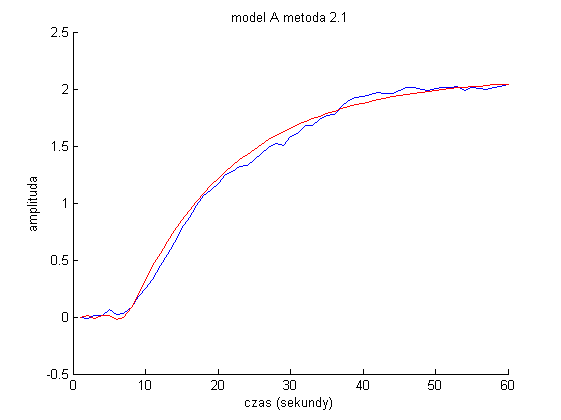
\includegraphics[width = \linewidth]{A_2_1}
\end{figure}

\end{frame}

% % % % % % % % % % % % % % % % % % % % % % % % % % % % % % % % % % % % % % % % % % % % % % % % % % % % % % % % % % % % %
\begin{frame}{Obiekt inercyjny I rzędu z opóźnieniem - Optymalizacja numeryczna }

\begin{equation*}
G(s) = \frac{k e^{-s \theta}}{T s + 1}
\end{equation*}

Parametry modelu dobrane z pomocą funkcji $fminsearch$:

\begin{itemize}
\item $\theta =  7.9828$
\item $k = 2.1475$
\item $T = 15.6379 $
\item błąd = 0.0015
\end{itemize}

\end{frame}


\begin{frame}{Porównanie modelu z obiektem rzeczywistym}

\begin{figure}
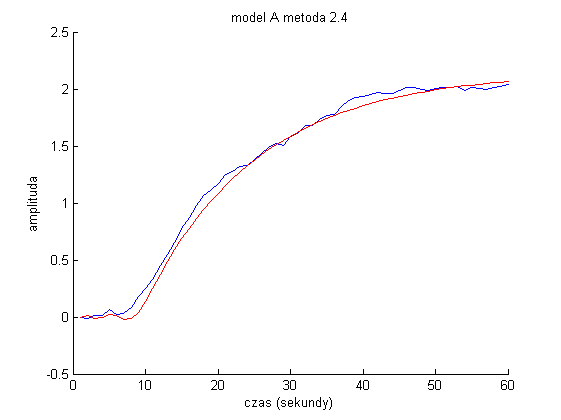
\includegraphics[width = \linewidth]{A_2_4}
\end{figure}

\end{frame}

% % % % % % % % % % % % % % % % % % % % % % % % % % % % % % % % % % % % % % % % % %
% % % % % % % % % % % % % % % % % % % % % % % % % % % % % % % % % % % % % % % % % % %
% % % % % % % % % % % % % % % % % % % % % % % % % % % % % % % % % % % % % % % % % % %

\begin{frame}{Obiekt inercyjny II rzędu z opóźnieniem }

\begin{equation*}
G(s) = \frac{k e^{-s \theta}}{(T_1 s + 1)(T_2 s + 1)}
\end{equation*}

Parametry modelu dobrane dobrane za pomocą metody I:

\begin{itemize}
\item $\theta = 7$
\item $k =  2.05$
\item $T_1 = 15.1515$
\item $T_2 = 1.51$
\item błąd = 0.0125
\end{itemize}

\end{frame}

% % % % % % % % % % % % % % % % % % % % % % % % % % % % % % % % % % % % % % % % % % % % % % % % % %

\begin{frame}{Porównanie modelu z obiektem rzeczywistym}

\begin{figure}
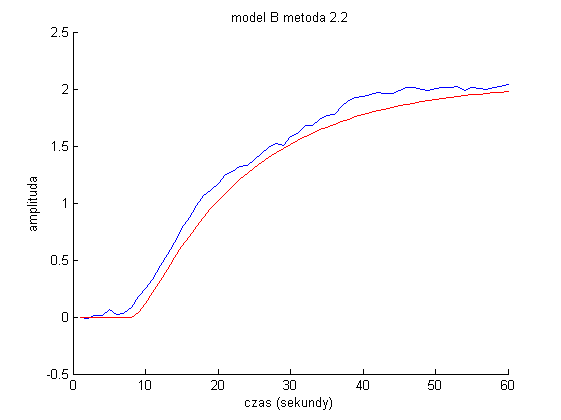
\includegraphics[width = \linewidth]{B_2_2}
\end{figure}

\end{frame}

% % % % % % % % % % % % % % % % % % % % % % % % % % % % % % % % % % % % % % % % % % % % % % % % % % % % % % % % % % % % %
\begin{frame}{Obiekt inercyjny II rzędu z opóźnieniem - Optymalizacja numeryczna }

\begin{equation*}
G(s) = \frac{k e^{-s \theta}}{(T_1 s + 1)(T_2 s + 1)}
\end{equation*}

Parametry modelu dobrane z pomocą funkcji $fminsearch$:

\begin{itemize}
\item $\theta =  5.2739$
\item $k =  2.1291$
\item $T_1 = 14.8349$
\item $T_2 = 2.0663 $
\item błąd =  0.0013
\end{itemize}

\end{frame}


\begin{frame}{Porównanie modelu z obiektem rzeczywistym}

\begin{figure}
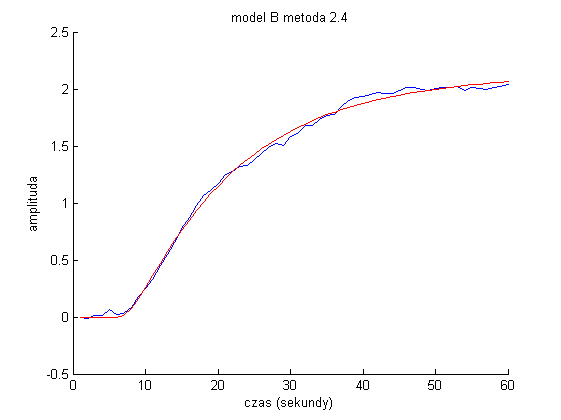
\includegraphics[width = \linewidth]{B_2_4}
\end{figure}

\end{frame}



% % % % % % % % % % % % % % % % % % % % % % % % % % % % % % % % % % % % % % % % % % % % % % % % % % % % % % % % % % % % %
\begin{frame}{Obiekt wieloinercyjny bez opóźnienia - Optymalizacja numeryczna }

\begin{equation*}
G(s) = \frac{k }{(T s + 1)^n}
\end{equation*}

Parametry modelu dobrane z pomocą funkcji $fminsearch$:

\begin{itemize}
\item $\theta =  6.6553$
\item $k =   2.0396$
\item $n = 3$
\item błąd =  0.0024
\end{itemize}

\end{frame}


\begin{frame}{Porównanie modelu z obiektem rzeczywistym}

\begin{figure}
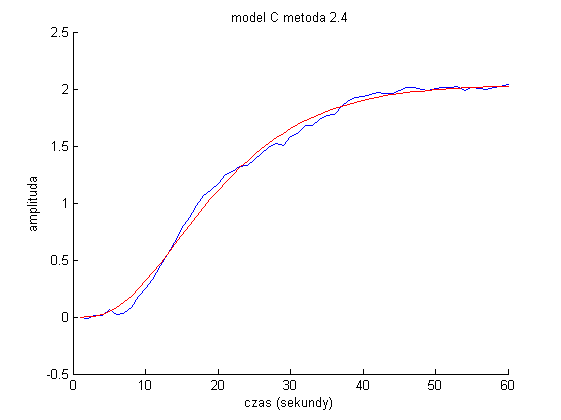
\includegraphics[width = \linewidth]{C_2_4}
\end{figure}

\end{frame}

\begin{frame}{Wnioski}

\begin{itemize}
\item Najmniejszy błąd średniokwadratowy uzyskaliśmy korzystając z modelu B(Obiekt inercyjny II rzędu z opóźnieniem) przy optymalizacji numerycznej. 
\item We wszystkich przypadkach metoda optymalizacji numerycznej dawała mniejsze błędy. 
\item Pozostałe metody opierały się na ,,ręcznej'' ocenie pewnych parametrów, co stwarzało pole do błędów
\end{itemize}


\end{frame}

\end{document}
